
\begin{theo}[Chapter Reference]{thm:pythagoras}
  The contents of the chapter is based on:
  \vspace{-0.4cm}
  \begin{itemize}
    \item Bayoumi, M., Nomidis, S. K., Willems, K., Carlon, E., and Maglia, G. (2021).
      Autonomous and active transport operated by an entropic dna piston.\\
      Nano Letters, 21(1):762–768. PMID: 33342212.
  \end{itemize}
  \vspace{0.3cm}
\end{theo}

The central topic of this is thee DNA nanopiston,  a molecular machine developed by the
Maglia research group[.]. The piston operates by turning over chemical fuel,
consisting of ssDNA,  into autonomous motion.

The design is based upon their earlier
work, where the group developed a protein rotaxane[.], consisting of a polypeptide thread
trapped in a Clya nanopore by two stopper proteins. This rotaxane could be moved between
two stable states inside the nanopore by an electric potential, acting as a molecular
switch.

This research lead to the development of the DNA nanopiston by Bayoumi et al.[.] in the
Maglia group. In this new molecular machine the rotaxane now constitutes of a DNA strand
instead of a polypeptide thread. Utilising the thermodynamic transitions of DNA, this
complex is capable of actively transporting DNA cargo-strands through the nanopore.

In this chapter the work of Bayoumi et al. is discussed, giving an overview of the
construction and operating cycle of this molecular machine.  At the end of this chapter
the molecular dynamics simulations from the paper of Bayoumi et al. are discussed, as
they where the main inspiration behind our project.

\section{Rotaxane Formation}


Synthetic molecular machines are often times embedded in larger complexes, providing the
necessary structure for their operation. For this reason biological nanopores are an
suitable starting point in the development of molecular machines. These transmembrane
proteins spontaneously self-assemble into well defined structures, embedded into a lipid
bilayer. Extensive research has been performed, designing methods and tools to tailor
their structural and electrostatic properties for specific use cases, originally focused
on Ionic current spectroscopy. This large back catalogue of research can now be employed
into building out their utility as an ideal building block for membrane bound molecular
machines.

The design of the DNA nanopiston is centred around the biological nanopore Cytolysin
A (ClyA). A modified variant ClyA-AS is used, which has been specially engineered for
use in Ionic Current Spectroscopy[.].


The nanopore is used to anchor a DNA Rotaxane structure inside the lipid membrane. The
large diameter of both its lumen and stem allows for the translocation of double
stranded DNA through the pore.



3. The DNA complex, built from three ssDNA sequences: ssDNA 1, ssDNA 2, and ssDNA 3.  The
last 70 bases of ssDNA 2 are complementary to the first 70 bases of ssDNA 1,  hence a
complex with neutravidin on one end, a 70-base dsDNA and two ssDNA overhangs on the other
end is formed, toehold. This complex is called the rotaxane.

2. The rotaxane is trapped in the nanopore by connecting it to two neutravidin stoppers
via biotin

The initial configuration is inspired by Ionic current spectroscopy. A clya nanopore
embeded on a lipid bilayer, seperating a saline liquid filed basin into two compartments.

To form the nanopiston Neutravidin (0.5 μM), ssDNA1 (5′-biotinylated, 100 bases, 1.2 μM)
and ssDNA 2 (80 bases,1 μM) were added to the cis solution. Applied a voltage of +100mV,
equal to a downward force on the analytes. The applied voltage induces an open pore
current through the pore, when the analytes enter the pore this blockage is measured.
The complex is trapped inside to pore indefinetely until the voltage is reversed.

While keeping the potential at +100 mV, the addition to the trans side of neutravidin (1
μM) and ssDNA 3 (3′-biotinylated, 20 bases, 2 μM), complementary to the last ten bases of
the ssDNA 1 overhang of the trapped thread. With the aim of reducing the free enrgy in
the system, the ssDNA strand hybridises will spontaneously hybridise with the other
strand. The completion of the hybridisation is checked by reversing the potential over
the pore, if the measured bloackage current remains the same it is assumed that the
hybridisation has occured and the rotaxane is formed.

\begin{figure}[ht]
  \begin{centering}
  \adjustbox{minipage=1.3em,valign=t}{\subcaption{}\label{sfig:testa}}%
  \begin{subfigure}[t]{\dimexpr.8\linewidth-1.3em\relax}
  \centering
  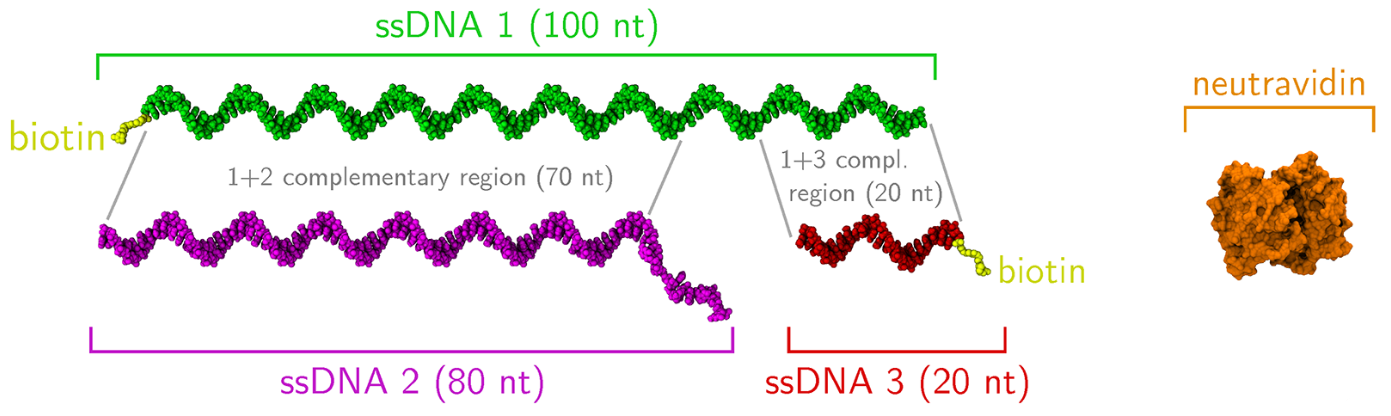
\includegraphics[width=\linewidth,valign=t]{Figures/RConstruction1.png}
  \end{subfigure}%
  \vspace{0.5cm}
  \adjustbox{minipage=1.3em,valign=t}{\subcaption{}\label{sfig:testa}}%
  \begin{subfigure}[t]{\dimexpr.8\linewidth-1.3em\relax}
  \centering
  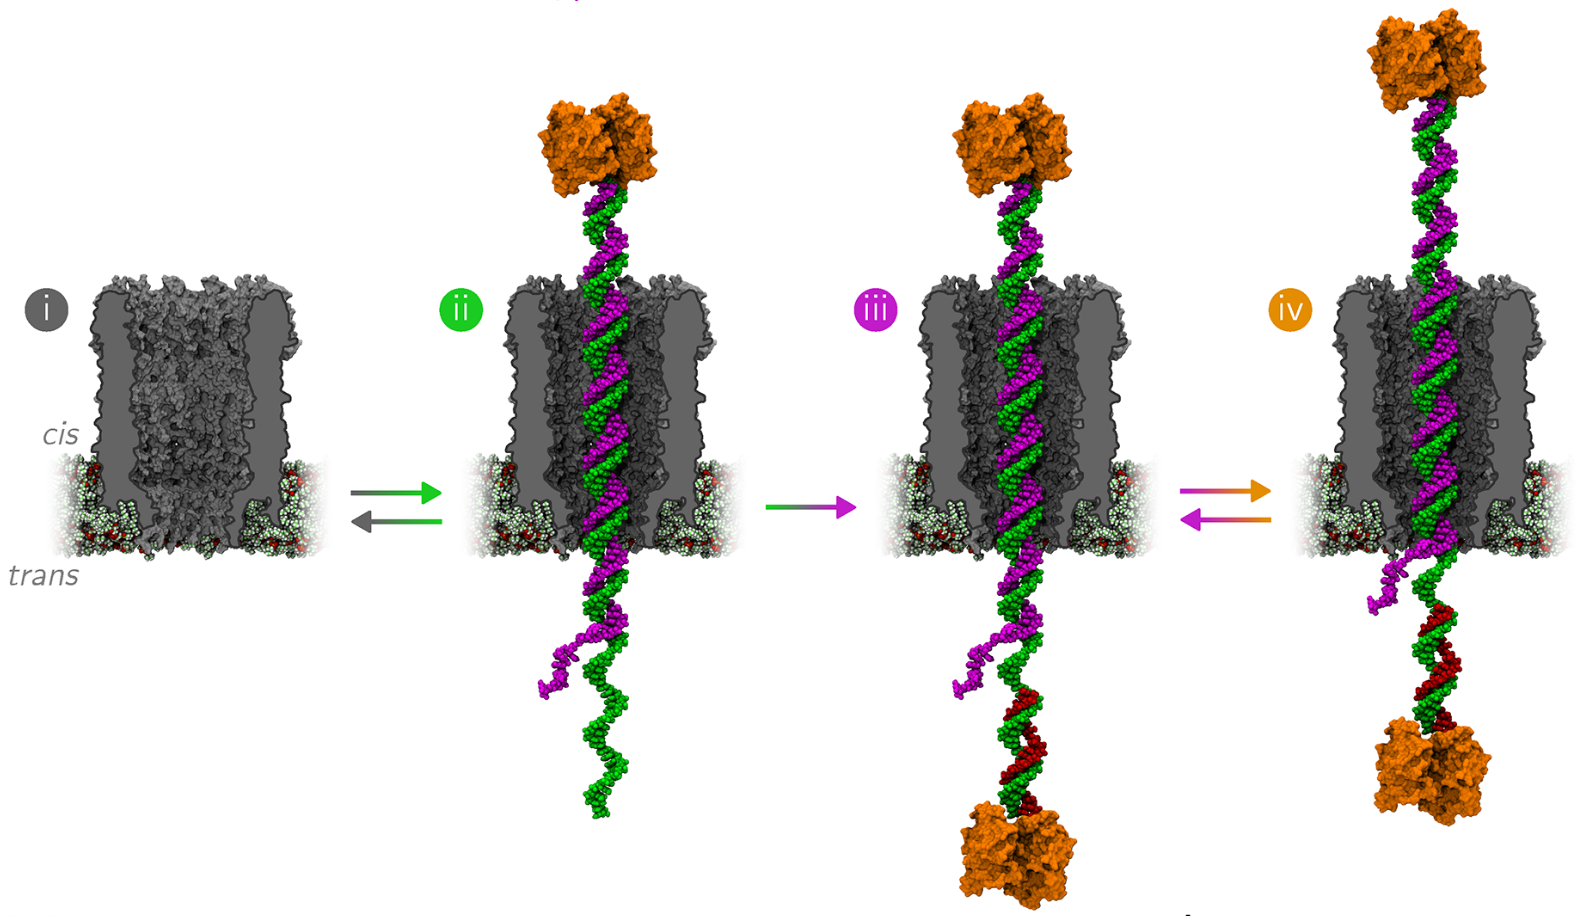
\includegraphics[width=\linewidth,valign=t]{Figures/RConstruction2.png}
  \end{subfigure}%
  \vspace{0.5cm}
  \adjustbox{minipage=1.3em,valign=t}{\subcaption{}\label{sfig:testb}}%
  \begin{subfigure}[t]{\dimexpr.8\linewidth-1.3em\relax}
  \centering
  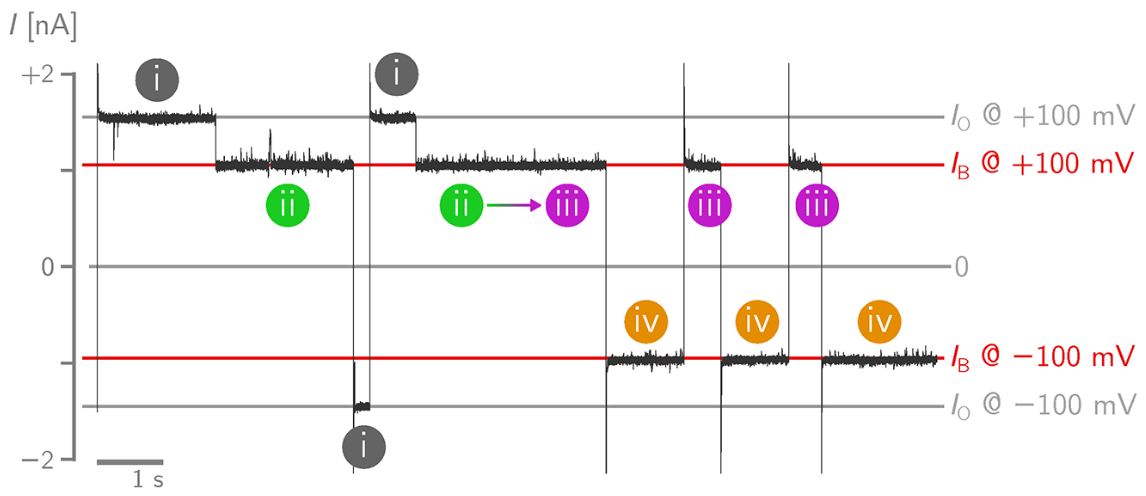
\includegraphics[width=\linewidth,valign=t]{Figures/RConstruction3.png}
  \end{subfigure}
  \caption{This is a figure [.]}
  \label{fig:test}
  \end{centering}
\end{figure}
